\documentclass[10pt]{article}
\usepackage[utf8]{inputenc}
\usepackage[T1]{fontenc}
\usepackage{amsmath}
\usepackage{amsfonts}
\usepackage{amssymb}
\usepackage[version=4]{mhchem}
\usepackage{stmaryrd}
\usepackage{graphicx}
\usepackage[export]{adjustbox}
\graphicspath{ {./images/} }

\title{PRESSURE AND INDUCTANCE EFFECTS ON THE VERTICAL STABILITY OF SHAPED TOKAMAKS }

\author{D.J. WARD, A. BONDESON, F. HOFMANN\\
(Centre de recherches en physique des plasmas, Association Euratom-Confédération Suisse, Ecole polytechnique fédérale de Lausanne, Lausanne, Switzerland)}
\date{}


\begin{document}
\maketitle
\section{LETTERS}


\begin{abstract}
Numerical calculations are presented to show the influence of pressure and inductance on the vertical stability of shaped tokamaks. High values of $\epsilon \beta_{p}$ improve the vertical stability of dee shaped tokamaks but are destabilizing for an inverse dee. For elongated cross-sections, the pressure effect is well described by a linear dependence of the maximum value of the stable internal inductance $l_{\mathrm{i}}$ on $\epsilon \beta_{\mathrm{p}}$, with a coefficient that depends on the geometry and increases with the triangularity. Stability diagrams are shown in terms of $l_{\mathrm{i}}$ versus $\epsilon \beta_{\mathrm{p}}$ for TCV- and DIII-D-like crosssections. Current profile effects depend critically on the wall configuration: low values of $l_{\mathrm{j}}$ are stabilizing if the wall is close, but increase the driving force of the instability in the absence of a wall. The competition between these two effects is considered for a configuration with discrete external conductors.
\end{abstract}

\section{INTRODUCTION}
Modern tokamaks are generally designed so as to take advantage of the increased current capability of an elongated cross-section and the resulting improvement of the beta limit [1,2] and confinement time [3]. A well known drawback of elongation is vertical instability $[4,5]$, which requires the use of conducting walls close to the plasma assisted by active feedback stabilization on the $L / R$ time-scale of the resistive wall. Work on the DIII-D tokamak has established that vertical instability is the factor that limits the achievable elongation [2, 6]. For the TCV experiment [7] in Lausanne, designed for a maximum elongation of $\kappa=3$, the vertical stability is a major issue, and we have therefore investigated numerically the operational limits due to the vertical instability and how these depend on, e.g., the shape of the plasma cross-section and the equilibrium profiles.

It is found experimentally [8] that the vertical stability of strongly elongated tokamaks is favoured by a low internal inductance $l_{\mathrm{i}}$, because this increases the coupling of the plasma current to the surrounding wall. Vertical stability requires an internal inductance less than some threshold value $l_{\mathrm{i}, \text { crit }}$, which decreases with\\
increasing elongation and wall distance. Here, we mean by $l_{\mathrm{i}, \text { crit }}$ the value of $l_{\mathrm{i}}$ for which a plasma surrounded by a realistic resistive wall has an $n=0$ growth rate, $\gamma_{\text {crit }}$, below which the vertical position can be controlled by a practical feedback system.

Our principal result is that $l_{\mathrm{i}, \text { crit }}$ is strongly influenced by pressure in combination with triangular shaping of the cross-section. We find numerically that $l_{i, \text { crit }}$ is an approximately linear function of $\epsilon \beta_{\mathrm{p}}$, independent of the details of the current profile and aspect ratio, but sensitively dependent on the geometry of the crosssection and the distance to the wall. For the usual dee shape, pressure is stabilizing, i.e. $l_{\mathrm{i} \text {, crit }}$ increases with $\epsilon \beta_{\mathrm{p}}$, whereas in an inverse dee, pressure is destabilizing. The increased upper limit in internal inductance for a normal dee is a favourable effect, not only because it makes it possible to reach a higher elongation, but also because the beta limit $[2,9]$ and confinement time [10] improve with the internal inductance at fixed elongation. Reference [2] shows convincing evidence that the optimum condition for reaching high beta is at the intersection of the $n=0$ and $n=1$ stability boundaries, where $n$ is the toroidal mode number.

The stabilizing effect of low inductance $l_{\mathrm{i}}$ is due to improved wall coupling in configurations with a completely surrounding wall. However, broad current profiles tend to give higher ideal growth rates with the wall at infinity. Here, we shall discuss the competition of these effects for a configuration where the wall is replaced by discrete conductors.

\section{STABILITY DIAGRAMS FOR TCV AND DIII-D CROSS-SECTIONS}
Figure 1 shows the limit in internal inductance $l_{\mathrm{i}, \text {, rit }}$ as a function of $\epsilon \beta_{p}$ for three different classes of current profiles in a 'TCV cross-section' at aspect ratio $A=1 / \epsilon=R_{0} / a=3.7$ (curves $1-3$ ). The following definitions are used for the poloidal beta:\\
$\beta_{\mathrm{p}} \equiv \frac{4}{\mu_{0} I_{\mathrm{p}}^{2} R_{0}} \int_{\mathrm{pt}} p \mathrm{~d}^{3} x$\\
and internal inductance\\
$l_{\mathrm{i}} \equiv \frac{2}{\mu_{0}^{2} I_{\mathrm{p}}^{2} R_{0}} \int_{\mathrm{p} \ell} B_{\mathrm{p}}^{2} \mathrm{~d}^{3} x$\\
The plasma-vacuum boundary is specified as\\
$R / a=A+\cos (\theta+\delta \sin \theta+\lambda \sin 2 \theta)$\\
$Z / a=\kappa \sin \theta$\\
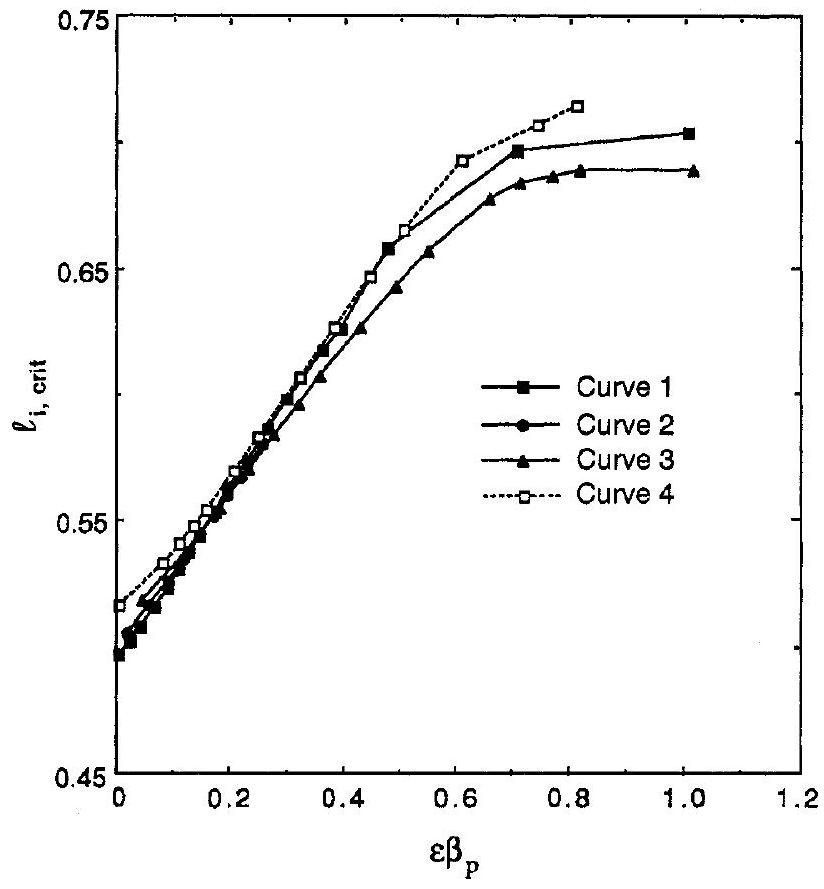
\includegraphics[max width=\textwidth, center]{2025_01_10_a0135324997886412d98g-3}

FIG. 1. Vertical stability diagram in terms of $1_{i, \text { crit }}$ and $\epsilon \beta_{p}$ for the TCV configuration. Curves $1-3$ show the results for the standard TCV configuration for three different types of current profiles. Curve 4 shows the results for the TCV plasma and wall shape expanded to an aspect ratio of $\mathrm{R}_{0} / \mathrm{a}=7.0$ for the first current profile.\\
and the geometry referred to as 'TCV dee' has elongation $\kappa=3$, triangularity $\delta=0.5$ and squareness $\lambda=0.2$. Equilibria have been computed with the CHEASE code [11] and stability with the NOVA-W code [12], which is capable of computing the growth rates of $n=0$ modes with a resistive wall, as well as with an ideal wall or with no wall. Figure 1 refers to resistive wall instabilities (cases that are stable with an ideal wall), and it is assumed that the mode can be stabilized by active feedback control if the resistive wall growth time is longer than $7 \%$ of the $L / R$ time of the wall (more precisely, for its ' $m=1$ ' eigenmode), i.e. 0.5 ms . The conducting wall represents the TCV vacuum vessel [7].

Several conclusions can be drawn from Fig. 1. Firstly, the limit in $l_{\mathrm{i}}$ is the same function of $\beta_{\mathrm{p}}$ for the three different classes of current profiles. The three current profiles differ significantly, and Fig. 2 shows the profiles 1 and 3 for the surface averaged toroidal current density $I^{*}$ at the point $l_{\mathrm{i}}=l_{\mathrm{i}, \text { crit }}$ at low and high pressures ( $\epsilon \beta_{\mathrm{p}}=0$ and 0.5 , respectively). (The pressure profiles have been chosen as uniformly scaled versions of those that give the ballooning limit with a\\
given $I^{*}$ profile.) Secondly, curve 4 refers to an equilibrium with a larger aspect ratio, $A=7$. The large aspect ratio result coincides almost exactly with that for $A=3.7$ when it is plotted in terms of $l_{\mathrm{i}}$ and $\epsilon \beta_{\mathrm{p}}$. Thus, for a fixed, elongated cross-section (but with varying current profile and aspect ratio) $n=0$ stability requires $l_{\mathrm{i}}<l_{\mathrm{i}, \text { crit }}\left(\epsilon \beta_{\mathrm{p}}\right.$ ), and for $\epsilon \beta_{\mathrm{p}}$ not too large $l_{\mathrm{i}, \text { crit }}$ is almost linear in $\epsilon \beta_{\mathrm{p}} ; l_{\mathrm{i}, \text { crit }} \approx l_{\mathrm{i}, 0}+c \epsilon \beta_{\mathrm{p}}$.

Figure 3 shows the corresponding result for a DIII-D-like cross-section, $\kappa=2.5, \delta=0.6, \lambda=0$ and $A=3$. Here, the resistive wall was chosen to be conformal to the plasma boundary, and two different minor radii have been considered for the wall; $d=1.3 a$ and $d=1.4 a$. The result is similar to that for the TCV dee shape in that the critical internal inductance increases with $\epsilon \beta_{p}$; however, the dependence is much stronger for the DIII-D cross-section. For the DIII-D-like case with $d=1.3 a$, we have $l_{\mathrm{i}, \text { crit }} \approx l_{\mathrm{i}, 0}+c \in \beta_{\mathrm{p}}$, with $c \approx 1.8$, which is much larger than for the TCV dee, where $c \approx 0.34$.

Also shown in Fig. 3 are two additional cases that compare the variation of the shape at the two different elongations. The first case has the high elongation ( $\kappa=3$ ) of the TCV dee shape, but with higher triangularity ( $\delta=0.6$ ) and no squareness $(\lambda=0)$. Because of the poor coupling of equilibria with this shape to the TCV vacuum vessel, we use a conformal wall with the distance chosen ( $d=1.275 a$ ) to give the same value of $l_{i, 0}$ as the TCV dee configuration at zero pressure. The stability boundary for this case has a slope almost as large as that for the DIII-D-like crosssection. The other case has the same elongation ( $\kappa=2.5$ ) as the DIII-D-like cross-section, but has the triangularity and squareness parameters corresponding to the TCV dee shape ( $\delta=0.5$ and $\lambda=0.2$ ). This case gives a line with an intermediate slope $c$ which is closer to that of the TCV dee shape. Thus, triangularity increases the slope and elongation decreases it, and in comparing the DIII-D and TCV dee shapes the effect of triangularity is dominant.

The stability threshold, of course, depends on the assumptions concerning the critical growth rate $\gamma_{\text {crit }}$. If the critical growth rate is changed, the main effect is a uniform shift of $l_{\mathrm{i}, \text { crit }}\left(\epsilon \beta_{\mathrm{p}}\right)$, with only a small effect on the slope $c$. For example, if $\gamma_{\text {crit }}$ for the TCV case, Fig. 1, is increased by $50 \%$ (this relaxes the demands on the feedback system), then the value of $l_{\mathrm{i}, 0}$ increases from 0.494 to 0.519 , while the slope $c$ increases by about $8 \%$. For the DIII-D-like case, if $\gamma_{\text {crit }}$ is increased by $50 \%$ the value of $l_{\mathrm{i}, 0}$ increases considerably, from 0.521 to 0.667 , but the value of the slope $c$ increases by only $3 \%$.\\
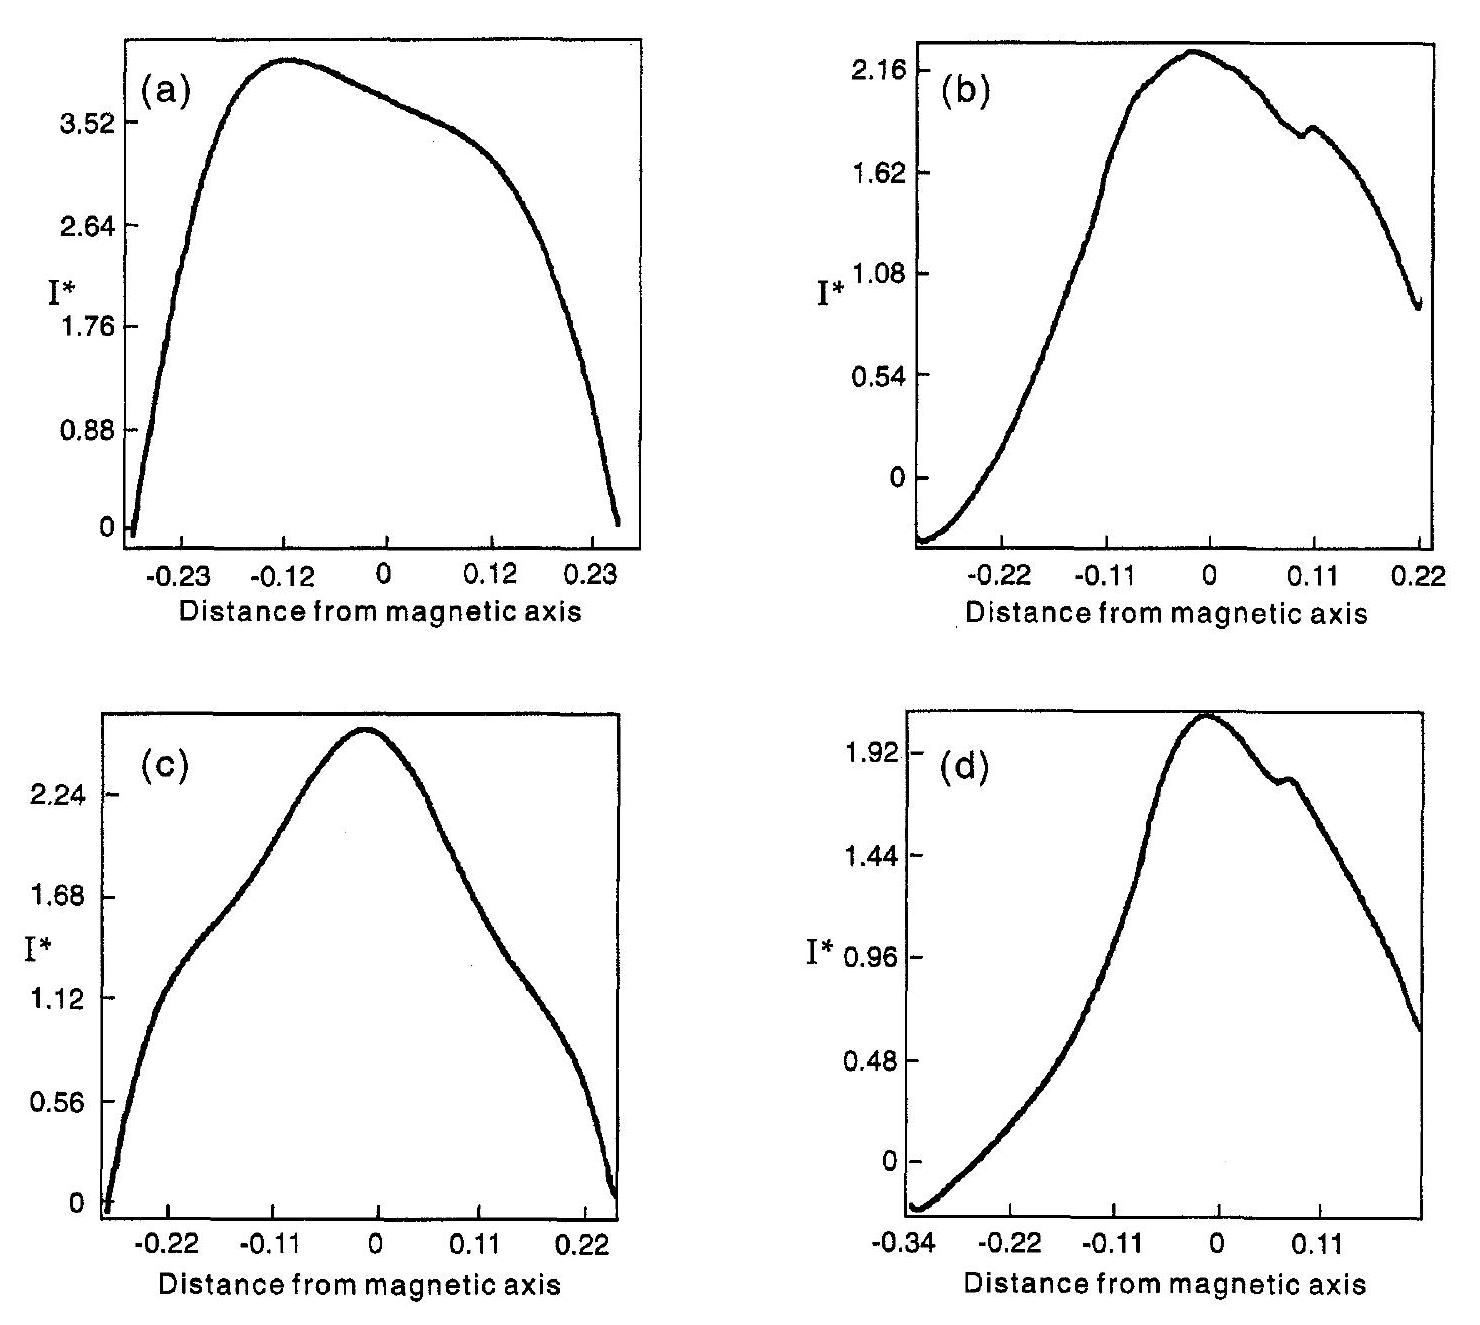
\includegraphics[max width=\textwidth, center]{2025_01_10_a0135324997886412d98g-4}

FIG. 2. Current profiles ( 1 * is the surface averaged toroidal current density) corresponding to curves 1 and 3 of Fig. 1. Both profile types are shown at low and high beta: (a) curve $1, \beta_{p}=0.06$; (b) curve $1, \beta_{p}=0.6$; (c) curve 3, $\beta_{p}=0.06$; (d) curve 3, $\beta_{p}=0.6$.

Note that Fig. 3 does not apply literally to DIII-D conditions, e.g. with respect to the assumed value of $\gamma_{\text {crit }} \tau_{\text {wall }}$. Furthermore, our definitions of $\beta_{\mathrm{p}}$ and $l_{\mathrm{i}}$ differ from those used in, for example, Ref. [2] by a shape dependent factor. For the DIII-D shape our values are smaller by a factor of approximately 1.5 . Improved vertical stability at high $\beta$ has been observed in DIII-D and was attributed to the broader current profiles at high $\beta$ due to a large fraction of bootstrap current [2]. Our calculations show that finite $\beta$ also has a direct effect on vertical stability, and this effect is significant for the DIII-D cross-section.

\section{BRIEF REVIEW OF THEORETICAL RESULTS}
Several results relevant to the diagrams in Figs 1 and 3 have been obtained previously by analytical [ $4,5,13-15]$, semi-analytical [16, 17] or numerical [18-20] methods. Quite surprisingly, most of the work on shape, pressure and inductance effects on vertical stability dates from the 1970 s, despite the subsequent development of powerful numerical codes and the fact that experiments are now in regimes where such effects are of importance.\\
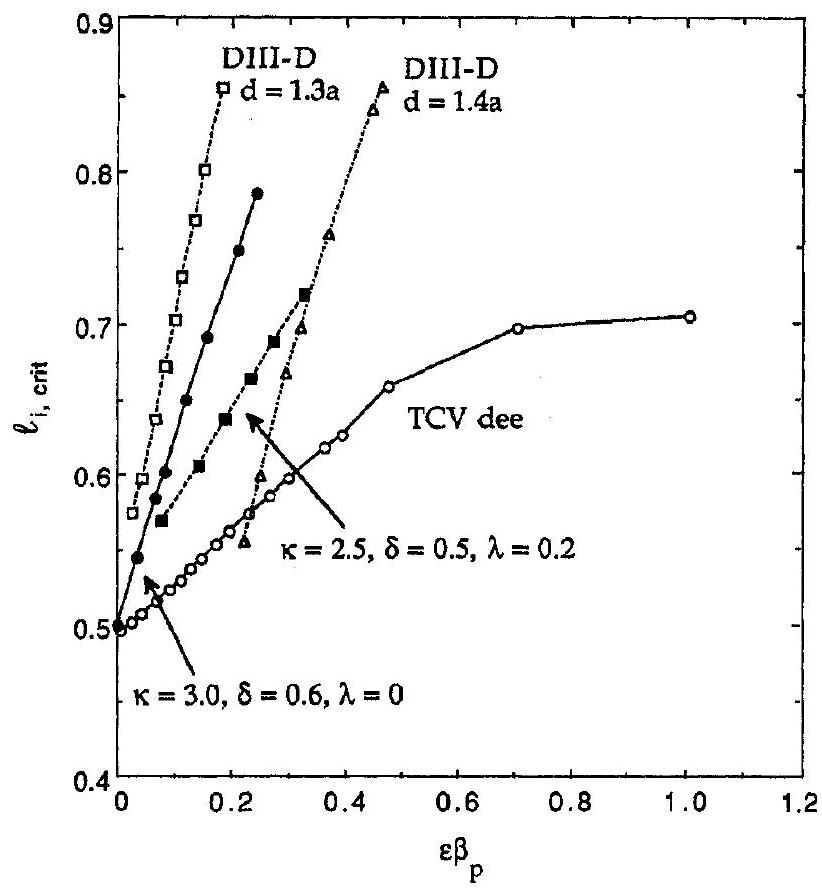
\includegraphics[max width=\textwidth, center]{2025_01_10_a0135324997886412d98g-5}

FIG. 3. Vertical stability diagram in terms of $1_{i, \text { crit }}$ and $\epsilon \beta_{p}$ for several equilibria of varying shapes. Two curves are shown for the DIII-D-like equilibrium with two different wall positions. The walls are conformal to the plasma shape at midplane distances of $\mathrm{d}=1.3 \mathrm{a}$ and $\mathrm{d}=1.4 \mathrm{a}$. For comparison, curve 1 from Fig. 1 for the TCV dee configuration is also shown. Two other stability boundaries intermediate between the DIII-D-like and the TCV dee equilibria are shown, with $\kappa=3.0, \delta=0.6, \lambda=0$ and with $\kappa=2.5, \delta=0.5, \lambda=0.2$.

Zakharov [4] showed that vertical elongation, $\kappa>1$, destabilizes vertical shifts but that a weakly elongated equilibrium can be stabilized by finite aspect ratio effects without the use of a conducting shell. Vertical displacements are stable if the decay index $n$ of the external vertical field satisfies $n \equiv-\left(R_{0} / B_{z}^{\text {ext }}\right)\left(\partial B_{z}^{\text {ext }} / \partial R\right)_{R=R_{0}}>0$.

Zakharov's expression [4,5] for $n$ implies that a plasma with a flat current profile is vertically stable when\\
$\kappa-1<\left(\frac{a}{R_{0}}\right)^{2}\left(\frac{3}{4} \ln \frac{8 R_{0}}{a}-\frac{17}{16}\right)$\\[0pt]
Laval et al. [13] showed that an elongated plasma can be stabilized by a conducting wall. For a flat current profile, their stability condition (in the near circular approximation) is\\
$\kappa-1<2\left(\frac{a}{d}\right)^{2}$\\
where $d$ is the wall radius. Comparison of the conditions (2) and (3) shows that for the elongations, aspect ratios and wall distances typical of modern tokamaks, wall stabilization is far more important than finite aspect ratio effects [21], and the discharges would be strongly unstable without a wall.

The effects of more complex shaping, including finite aspect ratio and pressure effects, were investigated semi-analytically for a surface current distribution by Rebhan and Salat [17]. For vertically elongated equilibria, they found that an inverse dee ( $\delta<0$ ) is destabilized by pressure, but a standard dee ( $\delta>0$ ) can be stabilized by pressure (see Fig. 4(a) of Ref. [17]). A stabilizing effect of finite pressure in combination with positive triangularity on the vertical stability of elongated equilibria is also indicated by the results [19] obtained with the ERATO stability code. This effect is the basic reason for the increased value of $l_{\mathrm{i}, \text { crit }}$ at high $\epsilon \beta_{\mathrm{p}}$ in the operational diagrams, Figs 1 and 3. The main new result shown in these diagrams is the appreciable size of the pressure effect on vertical stability in terms of the operational parameters, $l_{\mathrm{i}}$ and $\epsilon \beta_{\mathrm{p}}$, for more realistic current distributions than the surface current model of Ref. [17].

It has been shown $[14,18]$ that resistive wall growth rates (for equilibria that are unstable without a wall but stable with an ideally conducting wall) can be expressed in terms of the ideal MHD potential energies of the vertical shift mode in the absence of a wall, $\delta W_{\infty}$, and with an ideally conducting wall in the position of the resistive wall, $\delta W_{\mathrm{d}}$, as\\
$\gamma_{\mathrm{res}}=-\left(b / \tau_{\mathrm{w}}\right) \delta W_{\infty} / \delta W_{\mathrm{d}}$\\
Here, $\tau_{\mathrm{w}}$ is the $L / R$ time of the wall and $b$ is a numerical factor that depends on the current distribution in the wall. This expression gives valuable analytical insight. However, for numerical calculations it is more straightforward to introduce a resistive wall and solve the full eigenvalue problem as is done by NOVA-W. This automatically takes into account the effects of non-rigid displacements [22] and avoids the calculation of $\delta W_{\mathrm{d}}$ for a stable oscillatory mode which can be hidden by a continuous spectrum.

In the following two sections, we show the vertical stability results for ideal and resistive walls obtained with the NOVA-W code with the aim of placing the results for TCV dee and DIII-D cross-sections into a broader framework.\\
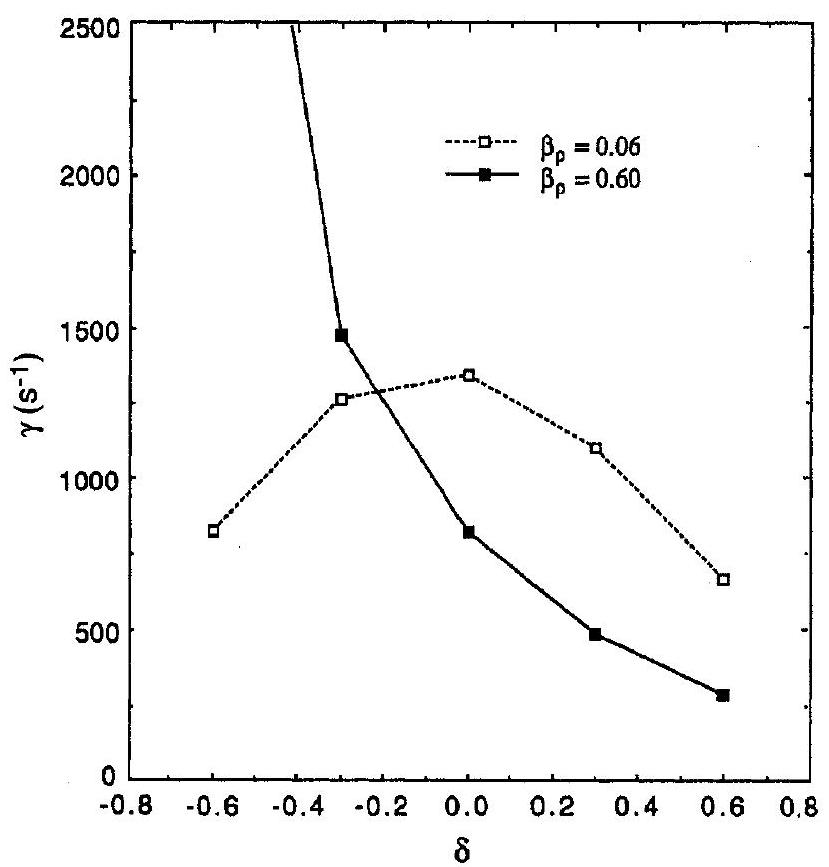
\includegraphics[max width=\textwidth, center]{2025_01_10_a0135324997886412d98g-6}

FIG. 4. Growth rates (in $\mathrm{s}^{-1}$ ) versus triangularity for a resistive wall conformal to the plasma shape at a midplane distance of $\mathrm{d}=1.3 \mathrm{a}$ for seversal shapes ranging from the inverse dee $(\delta=-0.6)$ to the regular dee $(\delta=0.6)$ at high beta $\left(\beta_{p}=0.6\right)$ and low beta $\left(\beta_{p}=0.06\right)$.\\
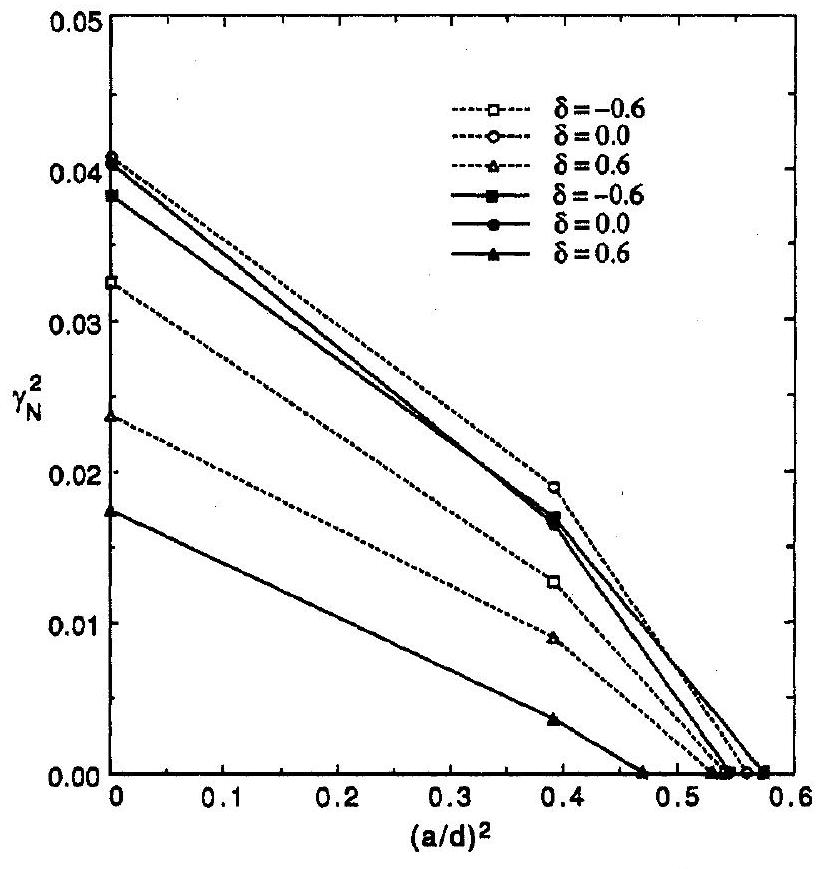
\includegraphics[max width=\textwidth, center]{2025_01_10_a0135324997886412d98g-6(1)}

F1G. 5. Plot of the square of the normalized ideal wall MHD growth rate $\gamma_{N}^{2}$ versus $\mathrm{a}^{2} / \mathrm{d}^{2}$, with an ideally conducting wall. The results are shown for three shapes (inverse dee, ellipse, regular dee) at high $\beta_{p}$ (solid symbols) and low $\beta_{p}$ (open symbols).

\section{PRESSURE EFFECTS}
The operational diagrams in Figs 1 and 3 show a much stronger stabilizing effect of $\epsilon \beta_{\mathrm{p}}$ in the DIII-Dlike cross-section ( $\kappa=2.5, \delta=0.6, \lambda=0$ ) than for the TCV dee shape ( $\kappa=3.0, \delta=0.5, \lambda=0.2$ ).\\
Figure 3 shows that the most important reason for this difference is the more triangular shape of DIII-D (note that a positive $\lambda$ decreases the effective triangularity [9]). The strong dependence of the pressure effect on triangularity is illustrated by Fig. 4. This figure shows resistive wall growth rates for elongated crosssections ( $\kappa=2.5, A=3$ ) at low and high pressures ( $\beta_{p}=0.06$ and 0.6 , respectively) and at several different triangularities ranging from $\delta=-0.6$ (inverse dee) to $\delta=+0.6$ (standard dee). The wall is a conformal copy of the plasma surface with minor radius $d=1.3 a$ and has the same resistivity and thickness as the TCV vacuum vessel used for Fig. 1. Pressure is strongly destabilizing for the inverse dee, somewhat stabilizing for the ellipse and clearly stabilizing for the standard dee. The inverse dee is strongly destabilized, and with $\beta_{\mathrm{p}}=0.6$ the mode is near marginal stability with an ideally conducting wall, see Fig. 5.

Figure 5 shows the square of the normalized ideal wall MHD growth rate (a measure of the ideal MHD driving energy) versus the reciprocal wall radius squared for three different triangularities ( $\delta=-0.6$, $0.0,0.6$ ) and for both high and low pressures. The dee shape is clearly the most stable among all the cases. For this configuration, a finite pressure is significantly stabilizing in the absence of a wall and remains so when wall stabilization is accounted for.

By contrast, for the inverse dee, pressure is clearly destabilizing both with and without a wall. The critical wall distance for the inverse dee is quite close to $d=1.3 a$, and therefore the resistive wall growth rate (with the wall at that position) is very large in Fig. 4 for that case. For the pure ellipse, the free space growth rate is virtually the same for the low and high pressure cases, but high pressure shows a stabilizing influence in the presence of a wall, and the growth rate falls below that for the inverse dee as the wall is moved inward.

Plots of the equilibrium flux surfaces show that, for the dee shape, increased pressure reduces the central elongation. This can be interpreted as the result of squeezing in the vertical direction by the combination of triangular shape and the Shafranov shift. The same effect leads to an increased elongation at high $\beta_{p}$ in an inverse dee.

\section{LETTERS}
We conclude that the primary effect of pressure on the dee shape is to lower the free space driving energy. Conversely, pressure increases the free space energy for the inverse dee. Thus, the favourable effect of pressure shown in the operational diagrams, Figs 1 and 3 , is mainly due to the lowering of the free space driving energy and not to its effect on the wall coupling. For the ellipse, the free space growth rates are virtually unaffected by pressure, but there is an increase in the wall stabilization for the high pressure case.

\section{CURRENT PROFILE EFFECTS}
It is well known that the current profile strongly influences the vertical stability. The almost identical results for different classes of current profiles in Fig. 1 show that the relevant parameter characterizing the current distribution is the internal inductance. Flat current profiles with low internal inductance lead to stronger coupling between the plasma and the external conductors. However, we find computationally that, in the absence of a conducting shell, the growth rate generally increases with decreasing inductance (see also Ref. [20]). This is shown in Fig. 6, where the ideal wall growth rate is plotted as a function of the wall radius for two DIII-D shaped equilibria with different internal inductances, $l_{\mathrm{i}}=0.6$ and 0.8 , respectively.

Peaking of the current profile is evidently stabilizing when the wall is distant but destabilizing when the wall is sufficiently close. At a wall distance of roughly $d=1.4 a$, the two curves in Fig. 6 cross, and the growth rate is independent of the inductance. This point is close to the critical wall distance. Therefore, the internal inductance has a rather small effect on the marginal position of the ideal wall, but it has a much stronger effect on the resistive growth rates with a close fitting wall [14]. In fact, with the wall at $d=1.3 a$, the two cases in Fig. 6 have nearly a factor of two difference in the resistive growth rate. The reduction of the free space growth rate with increasing inductance appears to be due mainly to a reduction of the ellipticity of the central flux surfaces. It should be noted that there are many competing effects, for example a similar reduction of the central triangularity, which reduces the finite pressure stabilization. In addition, peaking of the current profile effectively increases the aspect ratio, so that the toroidal stabilization is reduced. However, as discussed in Section 3, the toroidal stabilization is insignificant for highly elongated cross-sections.\\
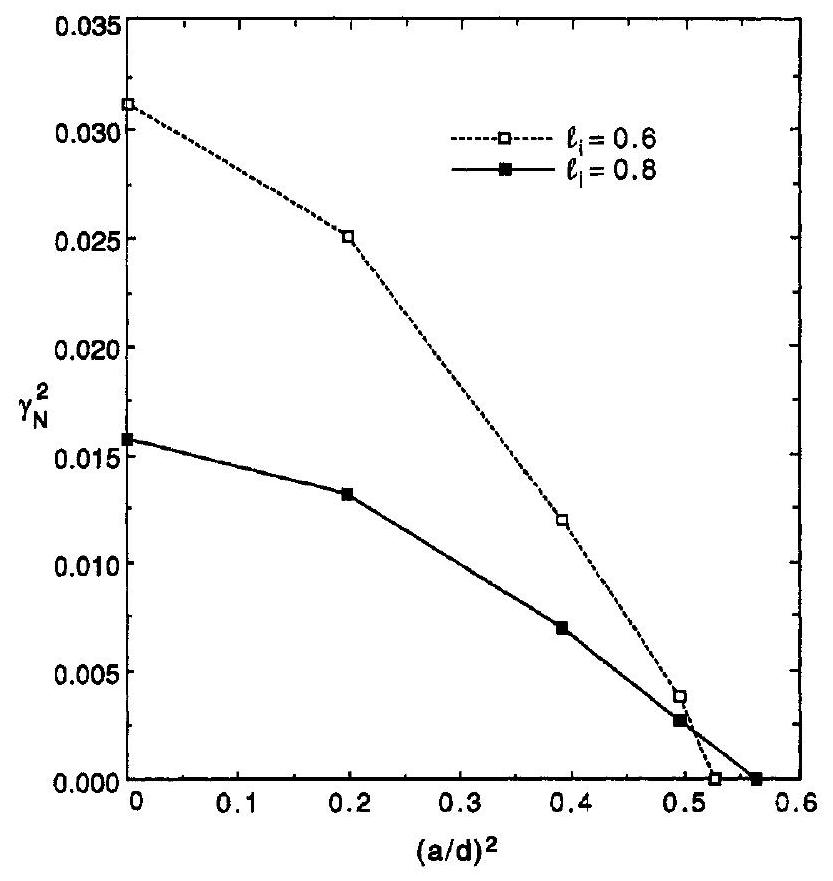
\includegraphics[max width=\textwidth, center]{2025_01_10_a0135324997886412d98g-7}

FIG. 6. Plot of $\gamma_{N}^{2}$ versus $\mathrm{a}^{2} / \mathrm{d}^{2}$ with an ideally conducting wall for DIII-D-like equilibria with no pressure for $1_{i}=0.6$ (dashed curve) and for $1_{i}=0.8$ (solid curve).

\subsection{Passive stabilization by discrete conductors}
While the effect of broadening the current profile increases the destabilizing force on the equilibrium, it also increases the stabilizing effect of a completely surrounding conducting wall. The balance between these competing effects is changed if the passive stabilization is provided primarily by discrete conductors instead of a complete, surrounding wall. As an example, we consider the configuration indicated in Fig. 7. The equilibrium has $\kappa=1.9, \delta=0.7$ and $A=4.54$. Figure 8 shows that in this configuration the growth rate increases with decreasing $l_{\mathrm{i}}$. This effect has been observed previously by Pearlstein [23] and by Jardin [24].

An interesting comparison is obtained by replacing the discrete conductors by the complete wall, as indicated by a dotted contour in Fig. 7. The total wall resistance was normalized to that of the passive conductors. Figure 8 shows that with the closed wall configuration the growth rate decreases monotonically with decreasing $l_{\mathrm{i}}$.

Figure 7 shows the contours of perturbed flux for the cases of (a) high and (b) low $l_{\mathrm{i}}$ in Fig. 8. While the coupling of the perturbed flux to the closed wall is\\
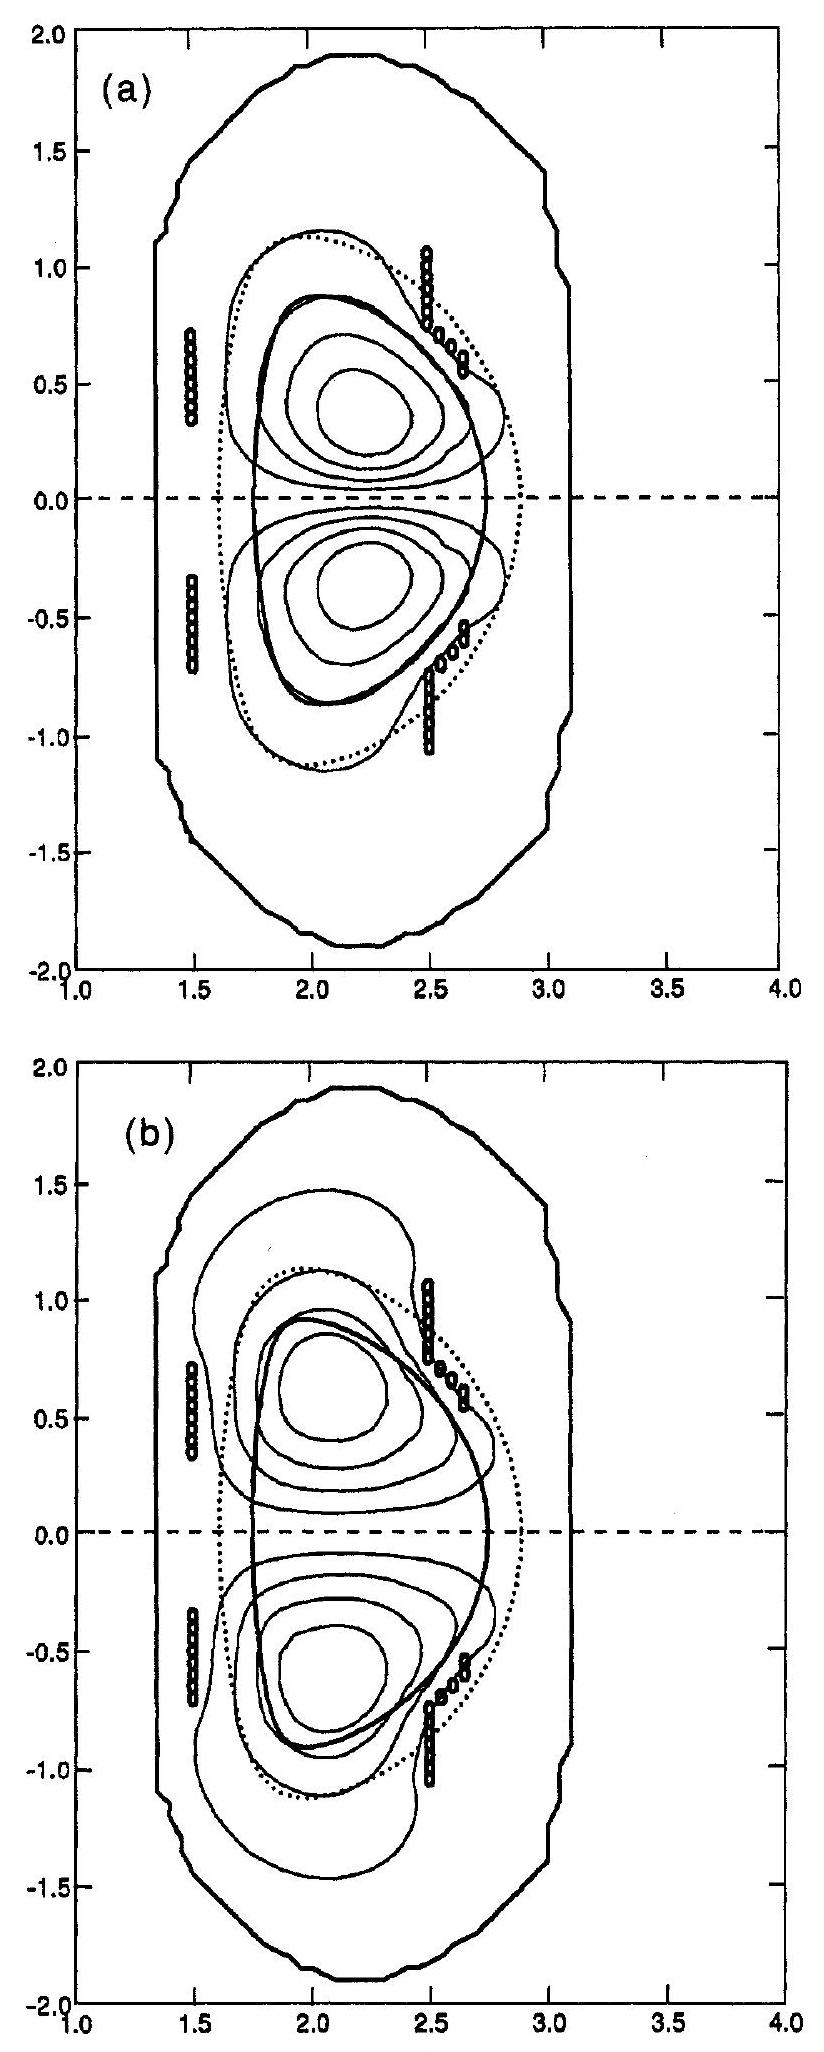
\includegraphics[max width=\textwidth, center]{2025_01_10_a0135324997886412d98g-8(1)}

FIG. 7. The plasma boundary, the discrete conductor sets and (shown as a dotted contour) a fictitious completely surrounding wall for the comparison in Fig. 8. The vacuum vessel is quite distant from the plasma. The perturbed flux contours are shown for two equilibria with (a) high $1_{i}$ and (b) low $1_{i}$ in the configuration with discrete conductors.\\
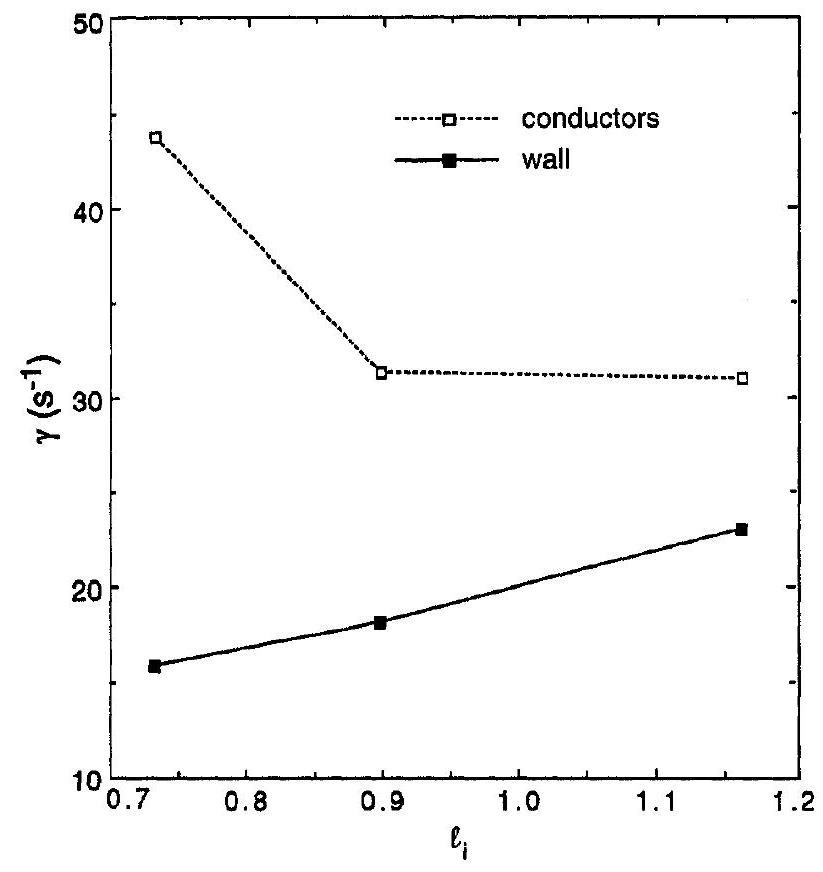
\includegraphics[max width=\textwidth, center]{2025_01_10_a0135324997886412d98g-8}

FIG. 8. Growth rates (in $s^{-1}$ ) versus $1_{i}$ for the configuration in Fig. 7 stabilized by discrete conductors with the vacuum vessel far from the plasma. For comparison, growth rates are shown with a completely surrounding wall (conformal to the plasma surface at $\mathrm{d}=1.3 \mathrm{a}$ ).\\
improved in the low $l_{i}$ case, the coupling to the discrete conductors is not. Therefore, the increase in the destabilizing force due to the broader current profile dominates, and the growth rate increases with decreasing $l_{\mathrm{i}}$.

We conclude that, for highly elongated tokamaks, there are two main effects of the internal inductance on vertical stability. Firstly, wall stabilization is improved for low internal inductance because of increased magnetic coupling. Secondly, current peaking reduces the shaping of the internal flux surfaces, which reduces the instability growth rate in the absence of a wall. For highly elongated, feedback stabilized discharges with a closed wall, the effect on wall coupling is more important, and stability improves at low inductance. However, when there is not a completely surrounding wall, the competition of these two effects is more subtle and depends on the details of the current profile and of the placement of the conductors.

\section{CONCLUSIONS}
We have found that high values of $\epsilon \beta_{\mathrm{p}}$ significantly improve the vertical stability of dee shaped tokamaks.

\section{LETTERS}
The effect can be described in terms of an almost linear dependence of the critical internal inductance on $\epsilon \beta_{\mathrm{p}}, l_{\mathrm{i}, \text { crit }} \approx l_{\mathrm{i}, 0}+c \epsilon \beta_{\mathrm{p}}$. Comparison between different cross-sections shows that the coefficient $c$ increases strongly with triangularity and decreases somewhat with elongation. For a DIII-D-like cross-section, the dependence of $l_{\mathrm{i}, \text { crit }}$ on $\epsilon \beta_{\mathrm{p}}$ is quite pronounced. This effect is beneficial for reaching high beta, because it increases the maximum stable elongation or, alternatively, allows the current profile to be more peaked, which increases the beta limit due to the $n=1$ external kink mode $[2,9]$.

\section{ACKNOWLEDGEMENTS}
This work was supported in part by the Swiss National Science Foundation. We acknowledge the work of H . Lütjens in adapting the CHEASE equilibrium code for NOVA-W.

\section{REFERENCES}
[1] TROYON, F., et al., Plasma Phys. Control. Fusion 26 (1984) 209.\\[0pt]
[2] LAZARUS, E.A., et al., Phys. Fluids B 3 (1991) 2220; LAZARUS, E.A., et al., Phys. Fluids B 4 (1992) 3644.\\[0pt]
[3] YUSHMANOV, P.N., et al., Nucl. Fusion 30 (1990) 1999.\\[0pt]
[4] ZAKHAROV, L.E., Sov. Phys. - Tech. Phys. 16 (1971) 645 (English translation: Zh. Tekh. Fiz. 41 (1971) 823).\\[0pt]
[5] MUKHOVATOV, V.S., SHAFRANOV, V.D., Nucl. Fusion 11 (1971) 605.\\[0pt]
[6] LAZARUS, E.A., et al., Nucl. Fusion 30 (1990) 111.\\[0pt]
[7] HOFMANN, F., et al., in Fusion Technology 1986 (Proc. 14th Symp. Avignon, 1986), Vol. 1, Pergamon Press, Oxford (1986) 687.\\[0pt]
[8] TAYLOR, T.S., et al., in Plasma Physics and Controlled Nuclear Fusion Research 1990 (Proc. 13th Int. Conf. Washington, DC, 1990), Vol. 1, IAEA, Vienna (1991) 177 ; LAO, L.L., et al., Phys. Fluids B 4 (1992) 232.\\[0pt]
[9] ERIKSSON, G., et al., in Plasma Physics (Proc. 1992 Int. Conf. Innsbruck), Vol. 16C, Part I, European Physical Society (1992) 343.\\[0pt]
[10] ZARNSTORFF, M.C., et al., in Plasma Physics and Controlled Nuclear Fusion Research 1990 (Proc. 13th Int. Conf. Washington, DC, 1990), Vol. 1, IAEA, Vienna (1991) 109.\\[0pt]
[11] LÜTJENS, H., et al., Comput. Phys. Commun. 69 (1992) 287.\\[0pt]
[12] WARD, D.J., et al., J. Comput. Phys. 104 (1993) 221.\\[0pt]
[13] LAVAL, G., et al., Phys. Fluids 17 (1974) 835.\\[0pt]
[14] HANEY, S.W., FREIDBERG, J.P., Phys. Fluids B 1 (1989) 1637.\\[0pt]
[15] ERIKSSON, H.G., Plasma Phys. Control. Fusion 34 (1992) 1721.\\[0pt]
[16] REBHAN, E., Nucl. Fusion 15 (1975) 277.\\[0pt]
[17] REBHAN, E., SALAT, A., Nucl. Fusion 16 (1976) 805.\\[0pt]
[18] HOFMANN, F., SCHULTZ, C.G., in Controlled Fusion and Plasma Physics (Proc. 16th Eur. Conf. Venice, 1989), Vol. 13B, Part I, European Physical Society (1987) 335.\\[0pt]
[19] BERNARD, L.C., et al., Nucl. Fusion 18 (1978) 1331.\\[0pt]
[20] BECKER, G., LACKNER, K., in Plasma Physics and Controlled Nuclear Fusion Research 1976 (Proc. 6th Int. Conf. Berchtesgaden, 1976), Vol. 2, IAEA, Vienna (1977) 401.\\[0pt]
[21] STAMBAUGH, R.D., et al., Nucl. Fusion 32 (1992) 1642.\\[0pt]
[22] WARD, D.J., JARDIN, S.C., Nucl. Fusion 32 (1992) 973.\\[0pt]
[23] PEARLSTEIN, L.D., Lawrence Livermore National Laboratory, personal communication, 1992.\\[0pt]
[24] JARDIN, S.C., Plasma Physics Laboratory, Princeton University, personal communication, 1992.\\
(Manuscript received 21 December 1992\\
Final manuscript received 29 March 1993)


\end{document}